% !TEX root =  master.tex
\chapter{Visualisieren der Daten (Phil Richter)}
Nach der Bereinigung und dem Speichern der Daten in einer Datenbank, wie in den vorherigen Kapiteln beschrieben, können die Daten visualisiert werden. Dafür wird als Grundlage
die Programmiersprache Python verwendet. Diese ist vorallem im Bereich der Datenanalyse und -visualisierung sehr weit verbreitet.

Für das Laden und Visualisiern der Daten werden folgende Packages verwendet:
\begin{table}[h!]
    \centering
    \begin{tabularx}{\textwidth}{|c|c|>{\centering\arraybackslash}X|}
        \hline
        \textbf{Package} & \textbf{Version} & \textbf{Beschreibung} \\ \hline
        dotenv & 1.0.1 & Lädt Umgebungsvariablen aus einer \textit{.env} Datei \\ \hline
        sqlalchemy & 2.0.36 & Ermöglicht Zugriff auf die Datenbank, sowie Datenbankabfragen \\ \hline
        pandas & 2.2.3 & Ermöglicht die Manipulation, Analyse und Verarbeitung von Daten \\ \hline
        matplotlib & 3.9.2 & Erstellt aus gegebenen Daten anpassbare Diagramme \\ \hline
        seaborn & 0.13.2 & Basiert auf \textit{matplotlib} und wird ebenfalls zur Datenvisualisierung verwendet \\ \hline
    \end{tabularx}
    \caption{Auflistung aller verwendeten Packages, sowie ihrer Versionen}
\end{table}

\section{Laden der Daten (Phil Richter)}\label{sec:laden}
Im ersten Schritt der Visualisieren werden die Daten aus der Datenbank geladen. Dafür werden die Datenbankverbindungsinformationen mit Hilfe von \textit{dotenv}
aus einer lokal definierten \textit{.env} Datei geladen. Anschließend wird mit \textit{sqlalchemy} eine Verbindung zur Datenbank aufgebaut und die Daten werden 
mit einer SQL-Querry abgefragt. Die abgefrageten Daten werden in einem \textit{pandas} DataFrame gespeichert. Ein DataFrame ist dabei eine zweidimensionale Datenstruktur,
wie eine Tabelle. Im folgendem Python-Code werden die Daten wie beschrieben geladen:

\lstset{
	breaklines=true,         % Enable line wrapping
	breakatwhitespace=false, % Allow breaks at any character (not just whitespace)
	basicstyle=\ttfamily,    % Use monospaced font
}

\begin{lstlisting}[caption={\texttt{load data from the database}},captionpos=b]
    import os
    import re
    import numpy as np
    import pandas as pd
    import seaborn as sn
    import matplotlib.pyplot as plt
    from sqlalchemy import create_engine
    from dotenv import load_dotenv

    load_dotenv() # load environment variables

    # get the environment variables
    b_user = os.getenv("DB_USER")
    db_password = os.getenv("DB_PASSWORD")
    db_name = os.getenv("DB_NAME")
    db_host = os.getenv("DB_HOST")
    db_port = os.getenv("DB_PORT")

    db_url = f"postgresql://{db_user}:{db_password}@{db_host}:{db_port}/{db_name}" # create the db url
    engine = create_engine(db_url)

    query = "SELECT * FROM intel;" # query to get the data from the database
    df = pd.read_sql(query, engine) # store the data in a dataframe
\end{lstlisting}

\section{Bereinigen der geladenen Daten (Phil Richter)}\label{sec:bereinigen}
Auch wenn die Daten, wie im Kapitel \ref{chap:säubern} beschrieben, bereits vor dem Speichern in die Datenbank bereinigt werden, bleinen kleine
Unreinheiten in den Daten bestehen. Daher werden bestimmte Spalten im DataFrame nochmals angepasst.

Ein Beispiel dafür ist die Spalte \textit{produktsortiment}. Diese enthält die jeweilige Generation des Prozessors, welche im Datensatz in drei verschiedenen
Schreibweisen vorkommt:
\begin{itemize}
    \item Die Generation als Zahl, z.B. \textit{4. Generation}
    \item Die Generation als Zahl ausgeschrieben, z.B. \textit{vierte Generation}
    \item Die Generation als englische Zahl, z.B. \textit{4th Generation}
\end{itemize}
Um die Prozessoren für die Visualisierung nach ihrer Generation Gruppieren/Sortieren zu können, wird die Spalte \textit{produktsortiment}
in eine neue Spalte \textit{generation} umgewandelt, wobei die Schreibweise vereinheitlicht wird. Dies wird mit Hilfe der Funktion \textit{extract\_generation}
gemacht. Der Code dazu sieht wie folgt aus:
\begin{lstlisting}[caption={\texttt{Funktion extraxct\_generation}},captionpos=b]
    number_words = {
        "erste": 1, "zweite": 2, "dritte": 3, "vierte": 4, "fuenfte": 5,
        "sechste": 6, "siebte": 7, "achte": 8, "neunte": 9, "zehnte": 10
    }

    def extract_generation(gen_text):
        # match the numeric generation
        match_numeric = re.search(r'(\d+)(?:\.|th)?\s?Gen', gen_text, re.IGNORECASE)
        if match_numeric:
            # return the numeric generation
            return int(match_numeric.group(1))
    for word, num in number_words.items():
        # check if the word is in the text
        if word in gen_text.lower(): 
            return num # return the number
    return None

    # extract the generation from the produktsortiment column
    df['generation'] = df['produktsortiment'].apply(extract_generation) 
\end{lstlisting}

Im Code wird zuerst ein Dictionary \textit{number\_words} definiert, welches die Zahlenwörter auf die entsprechende Zahl abbildet.
Anschließend wird die Funktion \textit{extract\_generation} definiert, welche einen String als Parameter erwartet und die Prozessor-Generation aus dem Text extrahiert.
Dabei wird zuerst mit Hilfe eines regulären Ausdrucks, faslls vorhanden, die numerische Generation extrahiert. Ein regulärer Ausdruck ist dabei eine Zeichenkette,
die ein bestimmtes Suchmuster für ein gegebenen String definiert.
Der in der Funktion verwendete reguläre Ausdruck "\textit{(\textbackslash d+)(?:\.|th)?\textbackslash s?Gen}" sucht nach einer Zahl gefolgt von einem Punkt oder \textit{th},
sowie einem Leerzeichen und den Buchstaben \textit{Gen}. Falls dabei ein übereinstimmender Text gefunden wird, wird dieser zurückgegeben. Anderenfalls wird
überprüft, ob eines der im Dictionary definierten Wörter im Text vorkommt. Falls ja, wird die entsprechende Zahl zurückgegeben.
Abschließend wird die Funktion auf die Spalte \textit{produktsortiment} angewendet und das Ergebnis in der neuen Spalte \textit{generation} gespeichert, welche nur noch die
Generation als Zahl enthält.
Die neue Spalte kann wie jede andere Spalte im DataFrame zur Visualisierung verwendet werden.

\section{Erstellen von Graphen (Phil Richter)}
Nachdem die Daten geladen und bereinigt wurden, können diese nun visualisiert werden. Dafür wird das Package \textit{matplotlib}, sowie \textit{seaborn} verwendet.
Diese sind sehr weit verbreitet und bieten eine Vielzahl an Möglichkeiten, um Daten zu visualisieren. Mit ihnen können verschiedene Diagramme wie Histrogramme,
Scatterplots, Balkendiagramme und viele mehr erstellt werden. Im folgenden ist ein Beispiel für ein Scatterplot und dessen Code dargestellt:

\begin{figure}[H]
	\centering 
	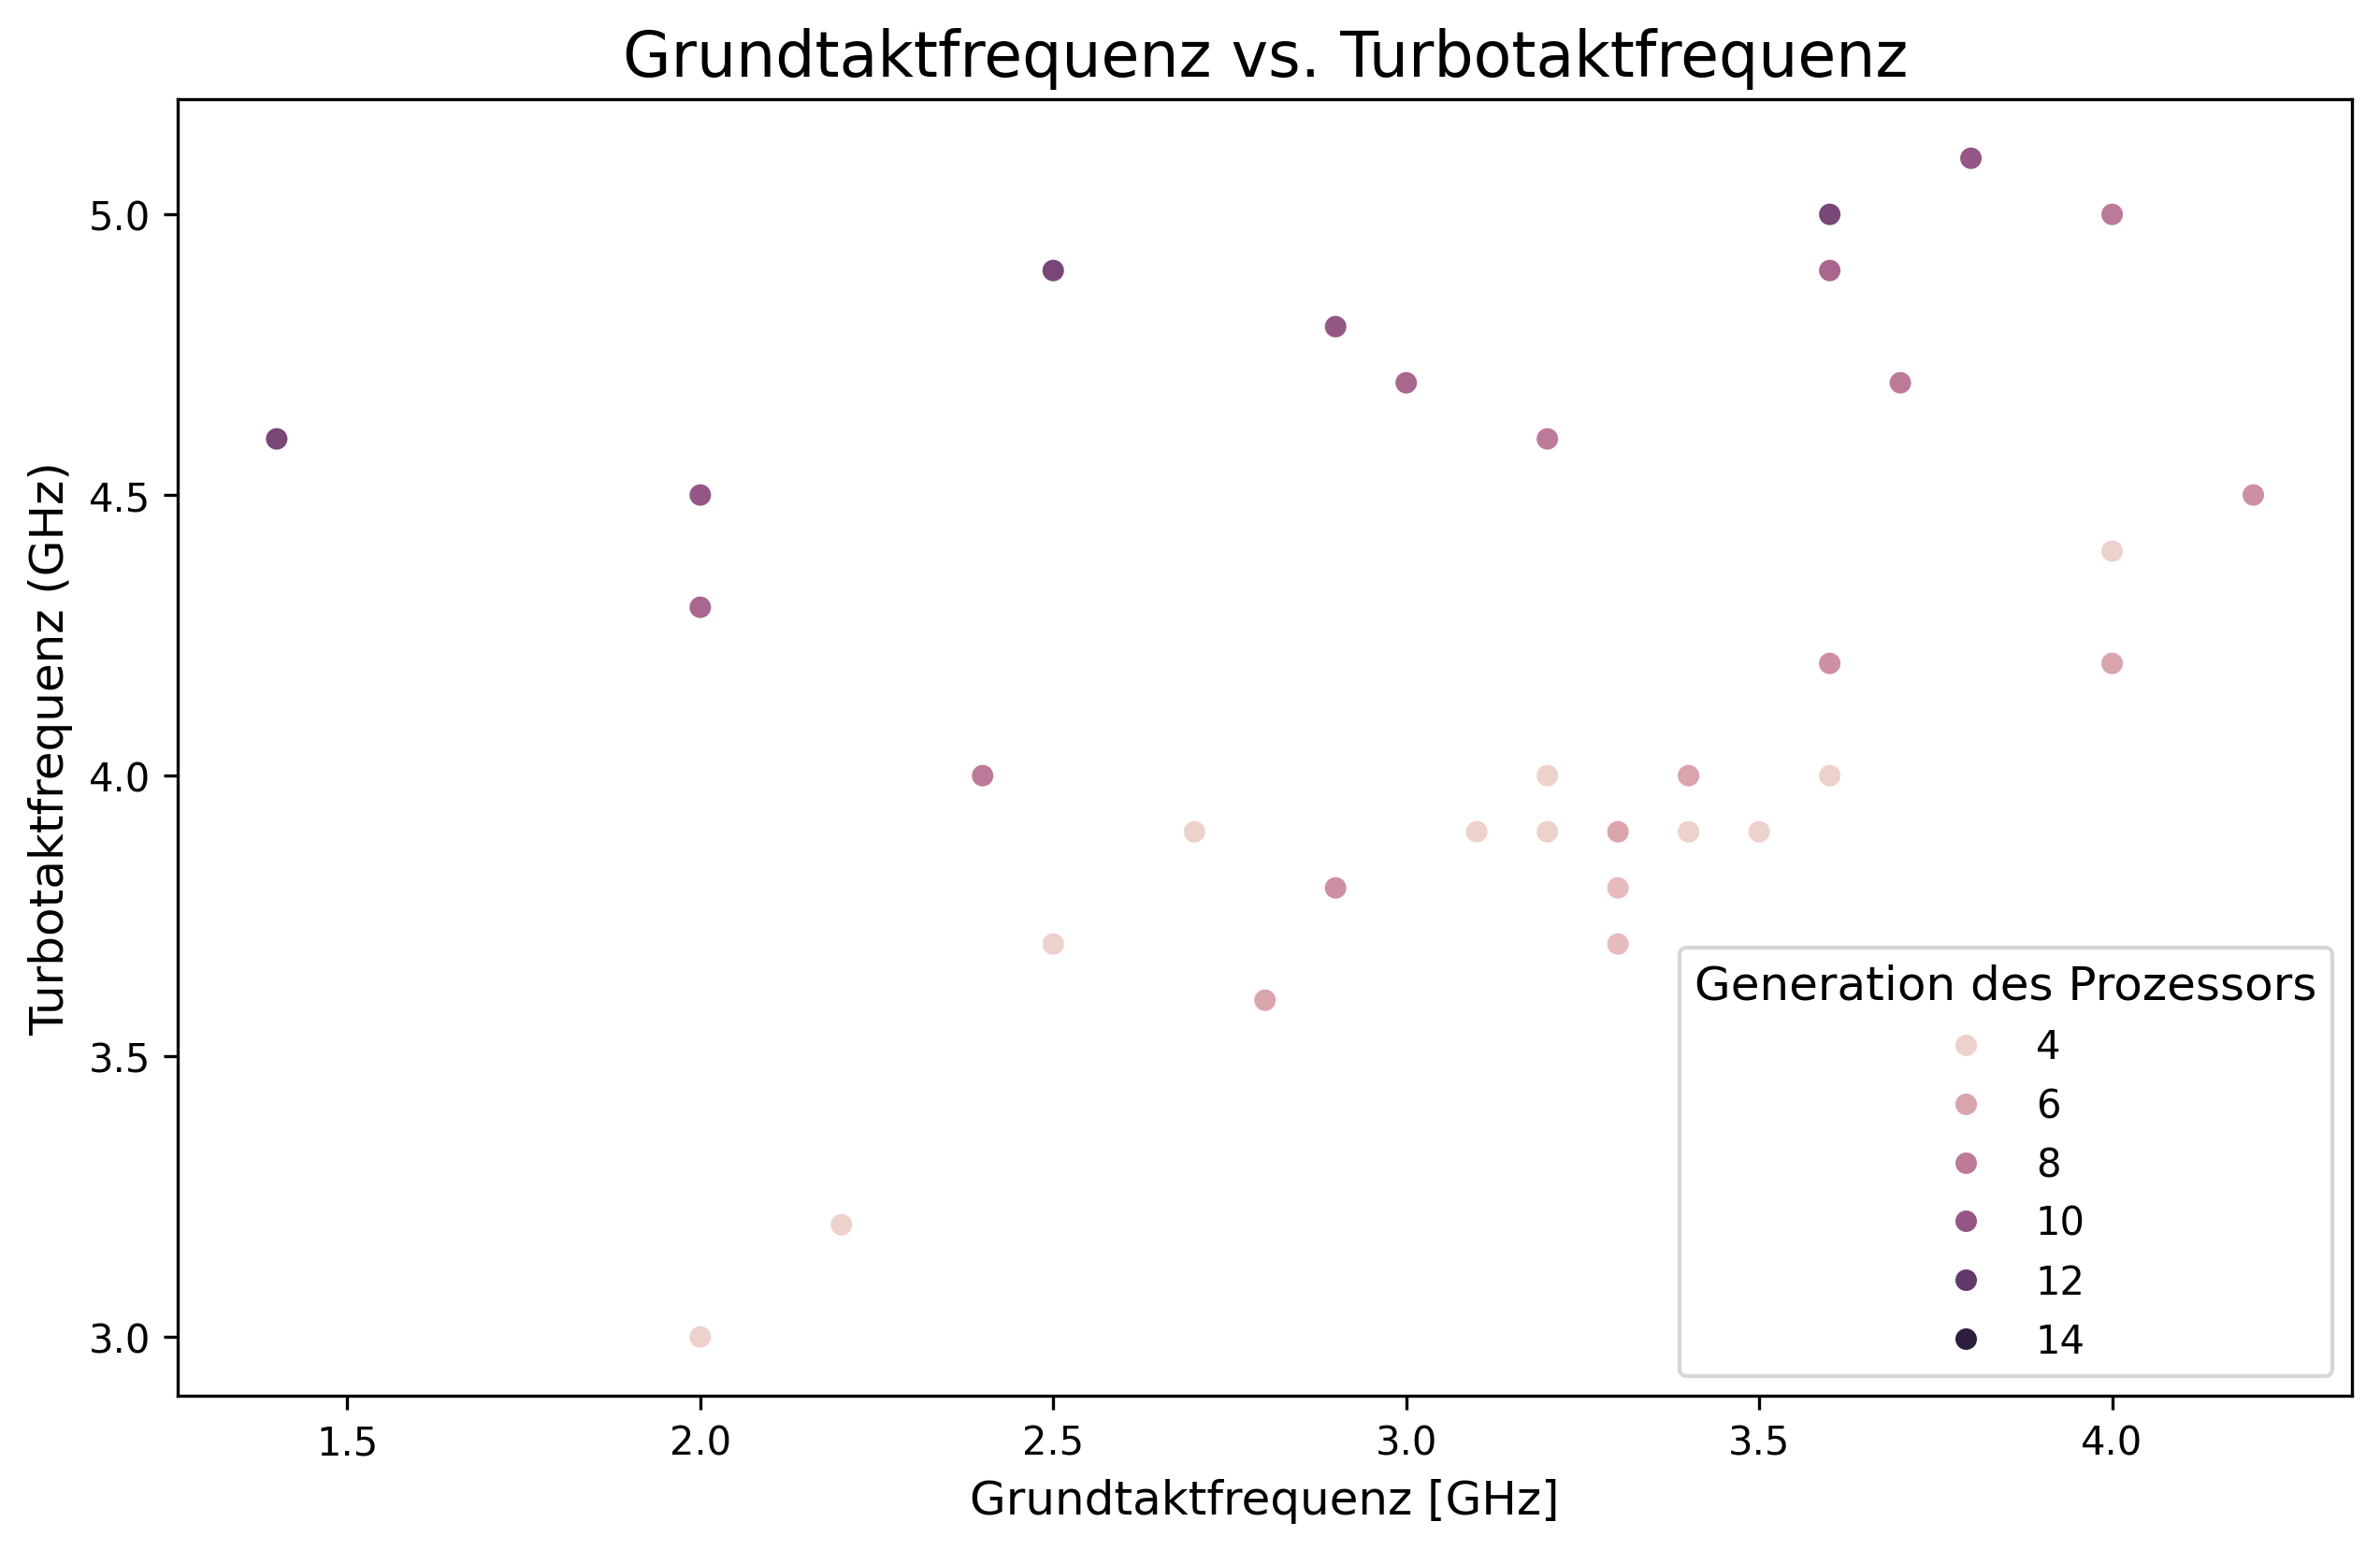
\includegraphics[width=\textwidth]{\imagedir/Scatterplot_Grundtaktfrequenz_vs_Turbotaktfrequenz.png} 
	\captionsetup{format=hang}
	\caption[Scatterplot]{\label{fig:scatterplot_Grundtaktfrequenz}Scatterplot erstellt mit \textit{matplotlib} und \textit{seaborn}}
\end{figure}

\begin{lstlisting}[caption={\texttt{Code für den Scatterplot in Figur 5.1}},captionpos=b]
    plt.figure(figsize=(10, 6))
    sn.scatterplot(data=df, x='grundtaktfrequenz_des_prozessors_GHz', y='max_turbo_taktfrequenz_GHz', hue='generation')
    plt.title("Grundtaktfrequenz vs. Turbotaktfrequenz", fontsize=16)
    plt.legend(title='Generation des Prozessors', fontsize=10, title_fontsize=12)
    plt.xlabel("Grundtaktfrequenz [GHz]", fontsize=12)
    plt.ylabel("Turbotaktfrequenz (GHz)", fontsize=12)
    plt.show()
\end{lstlisting}

Im Code wird zuerst ein neues Diagramm mit der Funktion \textit{plt.figure()} erstellt. Dabei wird die Größe des Diagramms auf 10x6 Zoll festgelegt. In Zeile
zwei wird mit der Funktion \textit{sn.scatterplot()} bereits der Scatterplot erstellt. Dabei wird als Datenquelle das im Kapitel \ref{sec:laden} erstellte DataFrame
\textit{df} verwendet. Die x-Achse wird mit der Spalte \textit{grundtaktfrequenz\_des\_prozessors\_GHz} und die y-Achse mit der Spalte \textit{max\_turbo\_taktfrequenz\_GHz}
belegt. Die Farbe des Punktes repräsentiert die Generation des Prozessors, welche in der im Kapitel \ref{sec:bereinigen} erstellten Spalte \textit{generation} gespeichert ist.
In den Spalten drei bis sechs werden der Titel, die Legende, sowie die Beschriftungen der x- und y-Achse festgelegt. Mit der Funktion \textit{plt.show()} in Spalte sieben wird
das Diagramm angezeigt.

Die restlichen Diagramme, die in dieser Arbeit erstellt wurden, sind nach einem ähnlichen Schema wie eben beschrieben erstellt worden. Dabei wurden unterschiedliche Diagrammtypen
sowie unterschiedliche Spalten des DataFrames verwendet. Alle Diagramme sind im Ordner \textit{Datenanalyse} in der Datei \textit{visualization.ipynb} zu finden.